% !TEX root = thesis.tex

% Front cover
% \includepdf{cover-front.pdf}

% Half-title
\maketitle


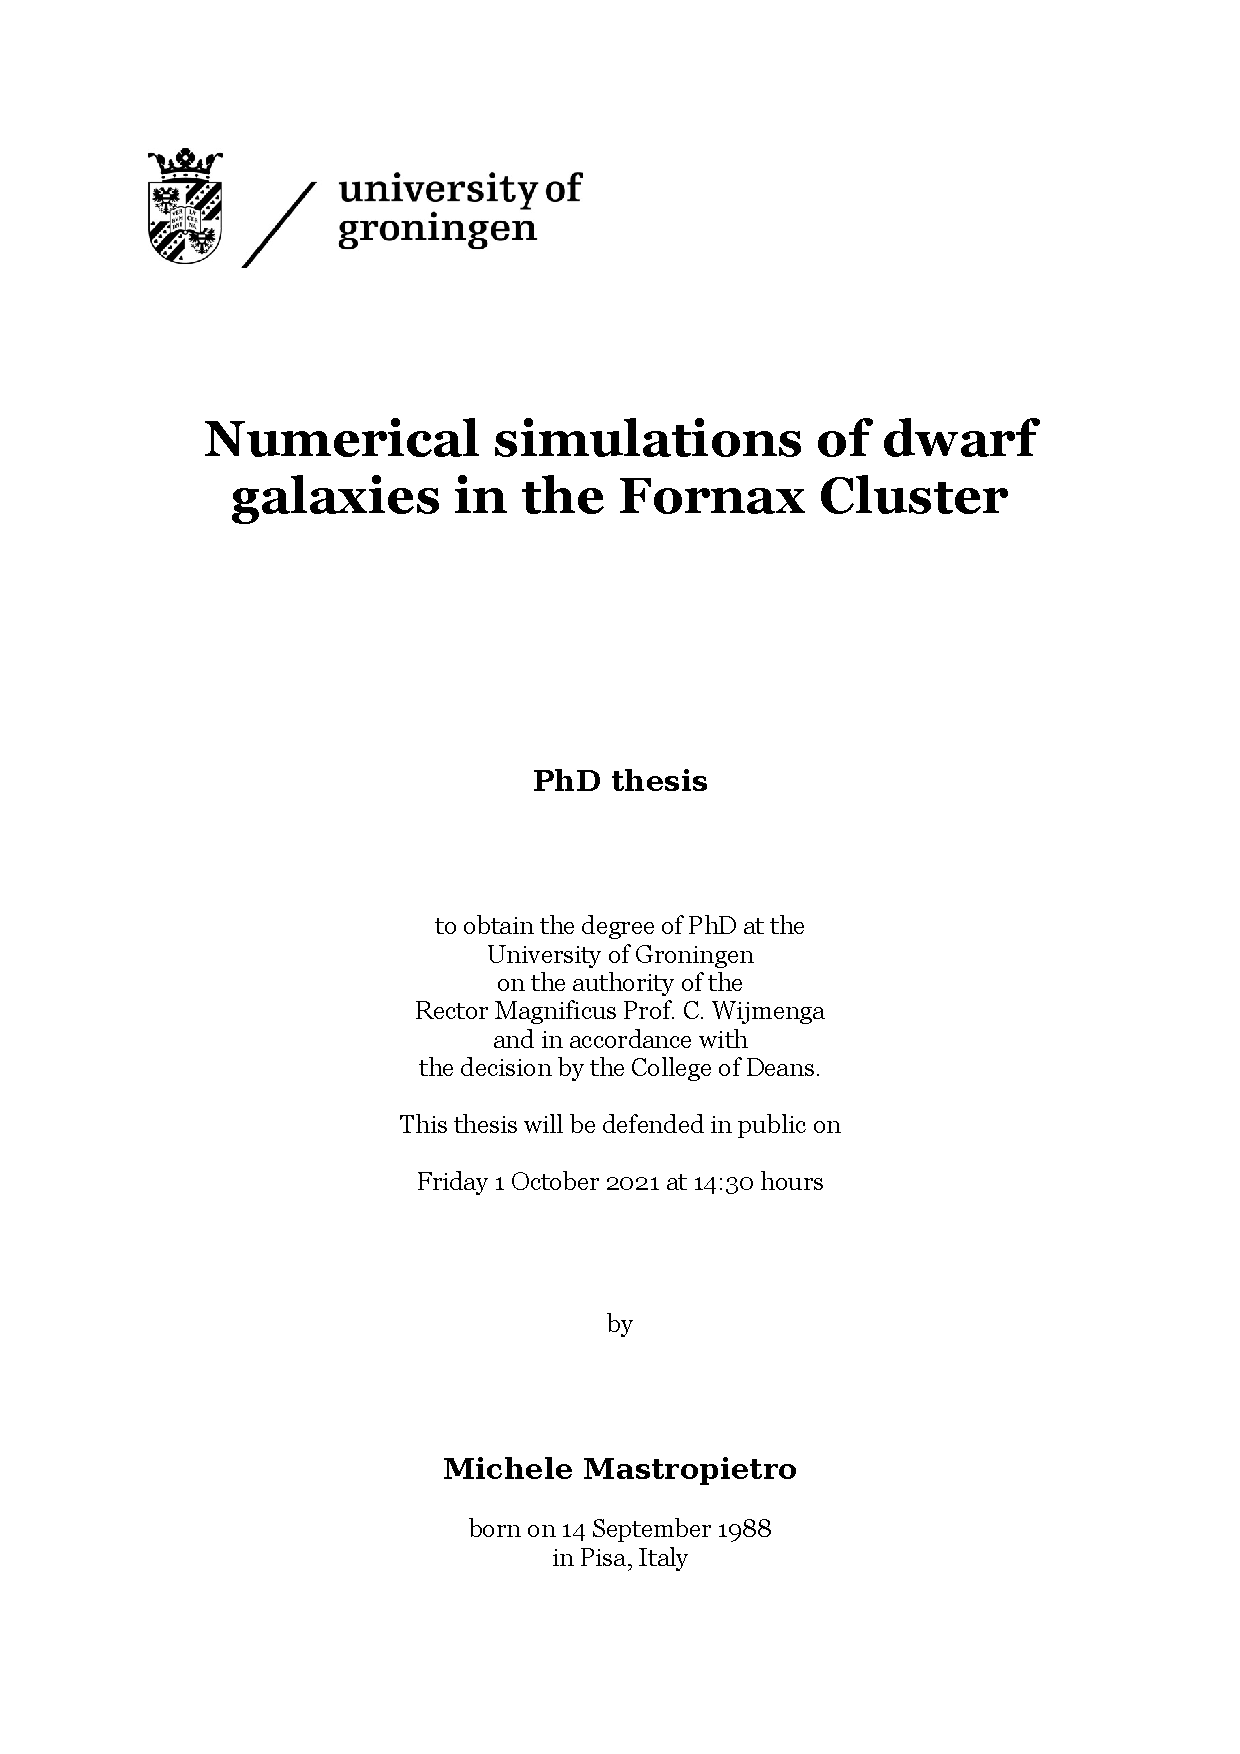
\includepdf[pages=-]{title_page.pdf}


\begin{comment}
% Official title
\begin{titlepage}
\null%
\label{thesis:title}
\vspace{3em}%
\pdfbookmark[1]{Title}{thesis:title}
\begin{center}

%% Skip space as in half-title
\vspace*{4\baselineskip}

%% Print the title.
\makeatletter
{\huge\@title}
\makeatother
\vfill

{\Large Proefschrift}

\medskip

{voorgedragen tot het behalen van \\
de graad van
Doctor in de Fysica en Sterrenkunde}


\medskip

door

\medskip

\makeatletter
{\Large \@author}
\makeatother

\medskip

aan de\\
{\large Universiteit Gent}\\
en aan de\\
{\large Rijksuniversiteit Groningen}\\
% Graduate School of Science and Engineering\\

\end{center}
\end{titlepage}





% Official verso
\clearpage
\thispagestyle{empty}
\null%
\label{thesis:committee}
\vfill
\pdfbookmark[1]{Doctoral committee}{thesis:committee}

% \noindent Members of the examination board:

\medskip\noindent
\begin{tabular}{@{}lll@{}}{Promotors:}\\\\
  \quad{}Prof.\ dr. Sven De Rijcke & Ghent University & (promotor)\\
  \quad{}Prof.\ dr. Michael\ Biehl & University of Groningen & (promotor)\\
  \quad{}Prof.\ dr. Reynier\ Peletier & University of Groningen & (promotor)\\
\\\\
\multicolumn{2}{@{}l@{}}{Composition of the Joint Evaluation Committee:} \\
\\
%   \quad{}Prof.\ dr.\  & chairperson \\
   \quad{}Prof.\ dr.\ Frazer Pearce & University of Nottingham\\
   \quad{}Prof.\ dr.\ Arjen van der Wel & Ghent University \\
   \quad{}Prof.\ dr.\ John McKean & University of Groningen \\
   \quad{}Prof.\ dr.\ Hugues Talbot & Université Paris-Saclay\\
\medskip\noindent
%   \quad{}Dr.\ & University of Groningen\\
% \\
% \multicolumn{2}{@{}l@{}}{Independent members:} \\
% \\
%   \quad{}Prof.\ dr.\ & University of Technology \\
%   \quad{}Prof.\ dr.\ & University \\
%   \quad{}Dr.\& University \\
% \\
% \multicolumn{2}{@{}l@{}}{Other member:} \\
% \\
%   \quad{}Dr.\ & ...\\
\end{tabular}
\end{comment}



% Copyright page
\clearpage
\thispagestyle{empty}
\null%
\label{thesis:colophon}
\vfill
\pdfbookmark[1]{Colophon}{thesis:colophon}
\noindent Written in 2021 by {\makeatletter{\@author}\makeatother}.\\
\textbf{Copyright}~\cczero{} The template for the layout of this thesis was inspired by my colleague Sam Verstocken who used the template of the dissertation of \href{ken.mx}{Ken Arroyo Ohori},
which was released into the public domain using the Creative~Commons~\cczero{}~code.
To view a copy of the \cczero{}~code, visit:\\\url{http://creativecommons.org/publicdomain/zero/1.0/}\\
\textbf{Colophon}
% This thesis was typeset with \XeTeX, Version 3.14159265-2.6-0.99998 (TeX Live 2017/Debian) using the \mbox{{\fanciestfont{}Feijoa}}, \texttt{GT Pressura} and $\mathrm{Asana\ Math}$ typefaces.
Most of the figures were created using \href{http://ipe.otfried.org/}{Ipe} (Copyright © 1993–2020 Otfried Cheong).
The source code of this thesis is available at: \\
\url{https://github.com/elehcim/phd-thesis}\\
\textbf{Cover}
...\\[2ex]
This research was funded by the European Union's Horizon 2020 research and innovation programme under the Marie Sk\l odowska-Curie
% Skłodowska-Curie
grant agreement N.~721463 to the \href{www.astro.rug.nl/~sundial}{SUNDIAL ITN network}.
\begin{figure*}[bh!]
  \centering
  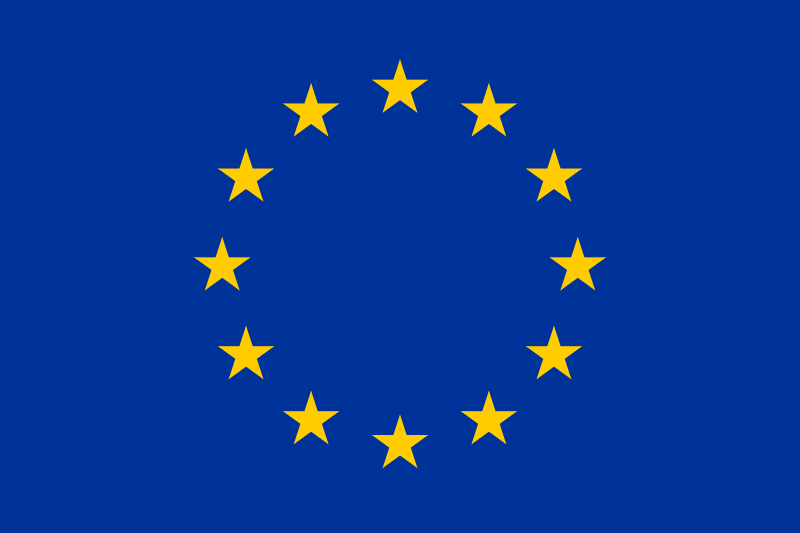
\includegraphics[width=0.2\textwidth]{EUflag}
\end{figure*}

% Aknowledgements page
\clearpage
\thispagestyle{empty}
\null%
\vfill
\begin{flushright}
  \textit{To my professor of physics:\\
      Mauro dell'Orso\\
      }
\end{flushright}
\vfill

% Aknowledgements page
\clearpage
\thispagestyle{empty}
\null%
\label{thesis:acknowledgements}
  \begin{center}
    {\Large \textbf{Acknowledgements}}\\
  \end{center}
\pdfbookmark[1]{Acknowledgements}{thesis:acknowledgements}
I'd like to thank first of all my professor Sven De Rijcke who believed in me doing a PhD in physics, since the first email in February 2017.
I thank you Sven for showing me what science is, how can it be beautiful and difficult and how it is a fantastic gym to train in deep honesty and integrity.
%As Feynmann said: we've learned from experience that the truth will come out, and it's this type of integrity, this kind of care not to fool yourself.
I've learned from you how to cope with work and life difficulties (especially in these pandemic times) in a very mature and ironic way.
Thank you also for being a mirror for me in our meetings, and always pushing me up even in my down moments.

The SUNDIAL project has been one of the nicest group of people I've ever met.
I'll never forget the high quality of people, their professionalism, attention and kindness for all of us. Thanks to prof. Michael Biehl, for your availability in this joint PhD journey.
Thank you prof. Reynier Peletier, our PI, practically a supervisor for all of us, always available to investigate new ideas with frank and direct attitude: %despite the many obligations and meetings you had to attend:
it's been very inspiring seeing how you live education of young scientists and astronomical research as a calling.
%Thank you Johan, my external mentor, for the interest you showed in my, for being kind and firm showing me how to clearly express.
Thanks to all of the ESRs, the one I had to work directly with: Marco, Abol, Bahar, and each one of the others: Maria Angela, Caroline, Aleke, Alex, Teymoor, Thanh, Mohammad, Shiv, Nushkia, Alan. All the best with your future.
The collaboration among us ESRs has often ended up in very good friendships, and I'll always remember the many memorable moments we lived together (in Naples, La Palma, Ghent...).

I thank my fellow astronomer colleagues at S9, the ones who are there, the ones who left during these years and the ones who just arrived.
I've learned so much from you academically and also how nice and beneficial is a happy work environment like the one you created.
The Belgian ``old guard": Maarten, Seba, Wouter, Peter, Sam, Marjorie, Dries, Robbert, Bert, Ilse, fellow Bert. Thank you for being so welcoming.
Thanks to Ana and Goran for the many moments shared together in our common expats life. Thanks to Francesco and Martina and their family: I've learned so much from you in these years we both were in Gent, much more than you think.
Caro and Pablo, thank you for all the support, deep sharing and friendship.Thank you dear office mates: Caroline, Sara, Anand and Yolan for the discussions and the nice coffee and fruit breaks.
You all have been so nice towards me, it's been an honour to work in the same place as you. Thank you for the many parties, events and dinners and many nice moments lived together.
I also thank the group of the Maxwell Demons: nice people for playing minivoetbal with fantastic team spirit.
Thank you Daniela and Andrea, young fellows of survival in lockdown times: I had so many great moments with you.
Thank you Shivangee, companion of the SUNDIAL adventure, of the office and of the life in Ghent in the happy moments as well as in the difficult times of the PhD far from home: for your constant positive attitude and for always asking how was going on for me and carefully listening. It meant a lot for me.
Thanks to Gianmarco (Jimmy), for showing me many times what true friendship means, and for being at the same time guest and host in our house in Belgium which became yours.
I thank Angelos, a real ``Sam" for me, in the sense of the Lord of the Rings: many times helping me %bringing the sometimes heavy burden of the PhD
and pulling me out of my down moments with frank conversations (is it a perk of living in Frank Baurstraat? ;P), sharing deep insights about life, cooking delicious Greek food (with an appropriate amount of garlic) and being the fuel of many parties and gatherings, with a lot of attention to everyone.

Thanks to my friends at Sint Jacobs in Gent: Davide and Ana (with the newly arrived Bea), Maria and Esteban (with the newly arrived Jose), Caique and Daniela, Valeria, Joshi, Pawel, Eligio and Luca: thank you for the improvised dinners, beers, holidays and deep friendship.
Many thanks to Pinco and the community of the Apostoline for helping me in many ways in these years: thank you for your wisdom and the constant example of free giving (gratuità profonda).

I thank my family: mamma e babbo, for your unbreakable, positive, caring attitude towards me.
%Mi stupisco spesso di come vi siate adattati a fare i genitori di persone adulte con i fatti mostrando una strada siate davvero i genitori che vorrei avere, in tutti questi anni.
Anto for the crystalline confrontations and the enormous sensitivity, Fra for the innumerable funny stories and deep thoughts. Nonna Lida per esserci ed essere una roccia salda per tutti, always.

%Looking back at these years and looking forward for what is waiting for me,
Now that the future opens up after this beautiful adventure of the PhD, I'm on the road to find out a good way to spend my life: each of you is invaluable for orienting me in this. Thank you!

\begin{flushright}
  Gent, 14th September 2021\\Michele Mastropietro
\end{flushright}

% Summary page
\clearpage
\thispagestyle{empty}
\null%
\label{thesis:Summary}
\begin{center}
  {\Large \textbf{Summary}}\\
\end{center}
\pdfbookmark[1]{Summary}{thesis:Summary}

\clearpage
\thispagestyle{empty}
\null%
\begin{center}
  {\Large \textbf{Samenvatting}}\\
\end{center}

\clearpage
\thispagestyle{empty}
\null%
\begin{center}
  {\Large \textbf{Riassunto}}\\
\end{center}